
%(BEGIN_QUESTION)
% Copyright 2015, Tony R. Kuphaldt, released under the Creative Commons Attribution License (v 1.0)
% This means you may do almost anything with this work of mine, so long as you give me proper credit

This pictorial diagram shows how a liquid level switch (with two separate SPDT switch units actuated by a common float mechanism) is wired to control both an electric pump and a lamp:

$$\includegraphics[width=15.5cm]{i02552x01.eps}$$

\begin{itemize}
\item{} Under what liquid level condition will the lamp energize?
\item{} Under what liquid level condition will the pump motor energize?
\item{} Determine what an AC voltmeter would register under the following conditions:
\begin{itemize}

\item{} Connected between terminals 2 and 6 ; low liquid level
\item{} Connected between terminals 4 and 7 ; low liquid level
\item{} Connected between terminals 1 and 6 ; high liquid level
\end{itemize}
\item{} Supposing the pump motor refused to energize but the lamp still functioned properly (turning on and off when it should), devise a series of diagnostic tests you could implement with an AC voltmeter to locate the fault.  For each test, explain what the result of that test {\it means} for your diagnosis of the problem.
\end{itemize}


\vskip 20pt \vbox{\hrule \hbox{\strut \vrule{} {\bf Suggestions for Socratic discussion} \vrule} \hrule}

\begin{itemize}
\item{} A problem-solving technique useful for analyzing circuits is to {\it re-draw the circuit} in a form that is easier to follow than what is shown to you on the given diagram.  Discuss and compare different renderings of this circuit, and how these simplified sketches help you with the analysis.
\end{itemize}


\underbar{file i02552}
%(END_QUESTION)





%(BEGIN_ANSWER)


%(END_ANSWER)





%(BEGIN_NOTES)

The lamp receives power through a NC (normally-closed) switch contact, which means it will be energized when the level switch is in the resting ({\bf low level}) state.

\vskip 10pt

The pump motor receives power through a NO (normally-open) switch contact, which means it will be energized when the level switch is in the actuated ({\bf high level}) state.

\begin{itemize}
\item{} Determine what an AC voltmeter would register under the following conditions:
\begin{itemize}

\item{} Connected between terminals 2 and 6 ; low liquid level -- {\it 0 VAC}
\item{} Connected between terminals 4 and 7 ; low liquid level -- {\it 120 VAC}
\item{} Connected between terminals 1 and 6 ; high liquid level -- {\it 0 VAC}
\end{itemize}
\end{itemize}

\vskip 10pt

The symptoms tell us the problem must be limited to the pump circuit, and cannot be related to anything common with both the pump and lamp, because the lamp still works as it should.  Taking a voltage measurement between terminals 6 and 7 while the liquid is at a high level is a good first step: the presence of 120 VAC between those points would indicate the switch is closing at it should, and that there must be an open fault between those terminals and the motor (including possibly within the motor itself).  The lack of voltage between those points during a high liquid level would indicate an open fault between those terminals the the source.

\vskip 10pt

Here are some indeterminate tests.  For each one, challenge students to explain {\it why} the specified test would not give good diagnostic information:

\begin{itemize}
\item{} Measuring voltage between terminals 1 and 2 ({\it We already know there is supply voltage, since the lamp works})
\vskip 5pt
\item{} Measuring voltage between terminals 6 and 7 while liquid level is low ({\it it is impossible for any fault prohibiting motor function to yield anything but zero volts in a condition of low level, and therefore this test tells us nothing about the problem})
\end{itemize}


%INDEX% Measurement, level: switch

%(END_NOTES)


